
\documentclass[journal,onecolumn]{IEEEtran}


\usepackage{parskip}
% *** GRAPHICS RELATED PACKAGES ***
%
\ifCLASSINFOpdf
  \usepackage[pdftex]{graphicx}

\else

\fi

% correct bad hyphenation here
\hyphenation{op-tical net-works semi-conduc-tor}


\begin{document}

% Title
\title{CSE 578: Data Visualization - Course Project}

% Author
\author{Andrey Sokolov}

\maketitle

\begin{abstract}
    This report presents an in-depth analysis of income-related factors to develop a
    marketing profile for UVW College. As part of our role at XYZ Data Company, we
    explored a dataset derived from the US Census Bureau, examining how various
    demographic and economic attributes influence whether an individual earns more than \$50,000 annually. 
    
    A comprehensive data pipeline was implemented, including data cleaning, feature
    selection, encoding techniques, and correlation analysis to identify the most
    impactful variables. Hierarchical clustering and principal component analysis
    (PCA) were utilized to reduce dimensionality and uncover hidden patterns.
    Multiple visualization techniques—such as stacked bar charts, heatmaps, and hierarchical clustering dendrograms—were applied to highlight key trends and relationships.
    
    Our findings indicate that factors such as marital status, occupation,
    education level, and hours worked per week exhibit the strongest correlations
    with income. Negative correlations with attributes like "relationship" and
    "sex" suggest structural influences that warrant further exploration.
    We also compared different classification models, evaluating decision trees,
    support vector machines (SVM), and neural networks for their predictive accuracy in income classification.
    
    The results of this study will inform UVW College’s enrollment and marketing strategies,
    allowing for data-driven decision-making. Future work includes refining predictive models,
    integrating additional socioeconomic data, and developing interactive visual tools to enhance usability for stakeholders.
    \end{abstract}

\section{Goals and Business Objectives}
XYZ Data Company is conducting an income-based analysis for UVW College to develop
a targeted marketing profile. The objective is to explore the influence of various
socioeconomic factors on an individual’s income level, specifically determining
whether they earn more or less than 50,000USD per year.

This analysis leverages data from the U.S. Census Bureau, including key attributes
such as education, occupation, marital status, and work hours per week. Through
data-driven visualizations and predictive modeling, this project aims to uncover
meaningful insights that will inform UVW College’s marketing and enrollment strategies.
By identifying trends and relationships between demographic characteristics and income,
we aim to help UVW College optimize its outreach efforts and target prospective
students more effectively.

\section{Assumptions}

\subsection{Technical Assumptions}
\begin{itemize}
    \item The dataset used for this analysis is representative of the overall population and contains minimal sampling bias.
    \item All missing values marked as `?` represent true missing data rather than meaningful categorical values.
    \item Python and its data science libraries (\texttt{pandas}, \texttt{seaborn}, \texttt{matplotlib}, \texttt{scikit-learn}) provide sufficient tooling to conduct this analysis.
    \item Data normalization or transformation will not be required unless strong skewness or inconsistencies are identified.
    \item The sample size is large enough to make meaningful observations about the data
    \item The categorical variables in the dataset can be meaningfully encoded without losing significant information.
    \item Outliers, if present, do not drastically impact results unless they are extreme and must be handled.
    \item The dataset structure (column names, data types) remains consistent throughout the analysis, ensuring no unexpected format changes.
\end{itemize}

\subsection{Business Assumptions}
\begin{itemize}
    \item Higher education levels are expected to correlate with higher income. Individuals with bachelor’s degrees or higher should have a greater likelihood of earning above \$50K.
    \item Binned age groups roughly correspond to life stages, for example 65+ for retirees
    \item We will sometimes use the relative term 'low' for a salary under 50K and 'high' for over 50K for ease of reading
    \item Marital status is assumed to be a strong predictor of income. Married individuals are expected to have a higher probability of being in the high-income group.
    \item Work class and occupation play a major role in income distribution. Higher-paying jobs (e.g., managerial roles, STEM careers) should show stronger income growth.
    \item Gender-based income disparities are likely to be present, with male individuals expected to have a higher proportion in the high-income bracket.
    \item Certain ethnic or national backgrounds might correlate with different income levels, potentially due to occupational clustering.
    \item Hours worked per week is expected to have a non-linear relationship with income, meaning that beyond a certain threshold, additional hours may not significantly increase earnings.
    \item Capital gains and losses are significant indicators of high-income individuals, particularly in investment-heavy occupations.
    \item The insights from this study can be generalized for UVW College’s marketing strategy, assuming that targeting specific demographic groups based on income factors will improve outreach effectiveness.
\end{itemize}
\section{Data Acquisition and Preprocessing}


\subsection{Data Cleaning Approach}
One of the initial challenges was ensuring the dataset was clean and structured correctly. The dataset contained missing values, inconsistencies in categorical variables, and redundant features. The steps taken were:
\begin{itemize}
    \item Removed 'fnlwgt' from DataFrame as it will not be used
    \item Identified and removed leading/trailing whitespace characters in multiple columns, identified by isolating unique values
    \item Checked for minimum and maximum of all continuous variables as well as any negative values. There are two maximums that seem to be capped - capital-gain(99999) and hours-per-week(99)
    \item Also identified missing values in the data, marked as '?'. These were replaced with 'None' as an indicator of missing values for Python interpretation
    \item Noted - number of missing values is quite low and only for a few variables - workclass and occuption(a correlated number) and native-country
\end{itemize}

\section{Feature Selection and Engineering}

\begin{description}
    \item[Q:] \textbf{Which attributes should be prioritized for analysis? How should they be chosen?}
    \item[A:] Initially, attribute selection was based on intuition and cursory data exploration. However, to ensure an evidence-based approach, correlation analysis and feature importance techniques should be applied. Attributes with strong correlations to income can be refined from preliminary machine learning models or manual EDA.

    \item[Q:] \textbf{What is the best algorithm to classify/model this kind of data? Decision Tree vs. SVM vs. Neural Network?}
    \item[A:] Several machine learning algorithms were considered and researched. A Decision Tree model seems like a good fit because it offers interpretability and handles categorical data well.

\end{description}

\section{Exploratory Data Analysis}

\subsection{Choosing the First Attributes for Analysis}
The first step in feature selection was identifying the most relevant attributes affecting income classification. The following approach was taken:
\begin{itemize}
    \item Conducted an initial exploratory data analysis to find at least one predictive attribute
    \item Selected \textbf{Education} as the primary attribute for early investigation, as it showed promising correlation with income level.
\end{itemize}

\subsection{Creating the First Visualization}
To validate early assumptions, the first visualization was created:
\begin{itemize}
    \item To plot salary versus education, we considered the binary nature of our key factor, salary. Since it is broken up into less than 50K and greater than 50K, it makes sense to plot using another attribute as an axis.
    \item Education is already broken up into integer values in the education-num category, but there are too many categories to comfortably display
    \item Therefore, we can consolidate the grade levels into one block, the non high school grad - this reduces down to 8 educational categories.
    \item Some thought was given to keeping associate degree (vocational) as "trade school", but outcomes are so similar to the traditional associate degree that it made more sense to combine the two
    \item Design Choices: Used distinct color coding for income categories, clear axis labeling, and a balanced layout for readability.
    \item Implementation: The visualization was created using Seaborn in Python.
    \item The aggregate visualization did a good job at representing the correlation between each education bracket and salary and clarity was further improved by sorting by education level left to right
\end{itemize}


\begin{figure}[h]
    \centering
    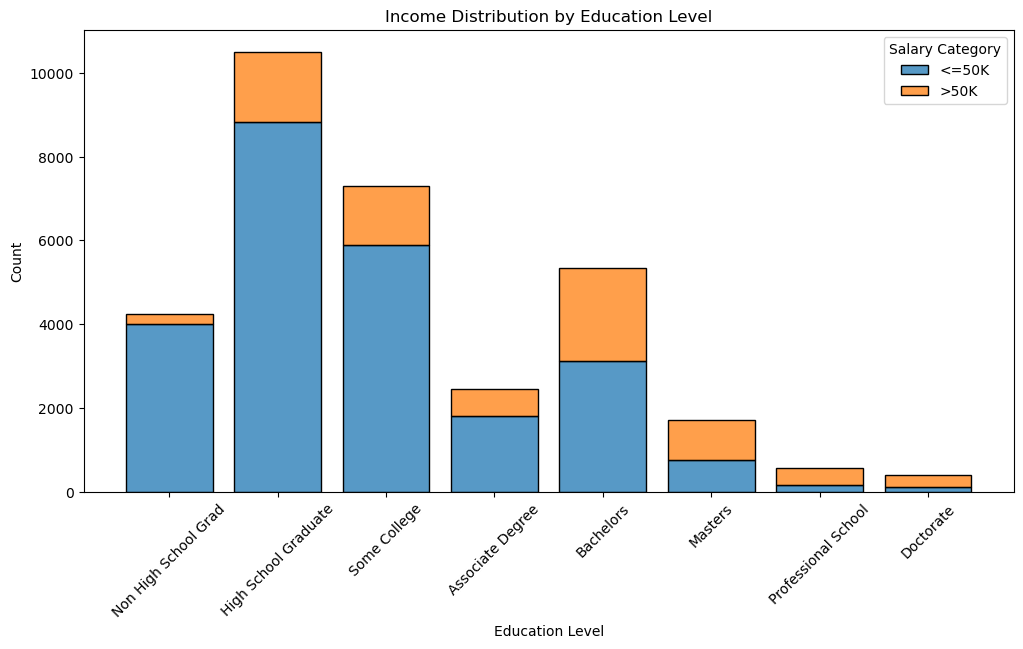
\includegraphics[width=0.9\linewidth]{hist_4.png}  % Reduce width slightly
    \caption{Final histogram for Income vs Education}
    \label{fig:final_income_vs_education}
\end{figure}
\section{Key Insights from Education Level vs. Income Distribution}

\begin{itemize}
    \item \textbf{Higher Education Correlates with Higher Income:} Individuals with advanced degrees (Masters, Professional School, Doctorate) have a significantly higher proportion of incomes above \$50K compared to those with lower educational attainment.
    
    \item \textbf{Most Common Education Levels:} The majority of individuals fall into the \textit{High School Graduate} and \textit{Some College} categories, making them the largest groups in the dataset. However, their income distributions do not show their education to be a predictor for the less than \$50K and greater than \$50K groups.
    
    \item \textbf{Education Alone is Not a Sole Predictor of Income:} Even at the Bachelor's level, a substantial number of individuals still earn less than \$50K. This suggests that additional factors such as work class, occupation, and experience must be considered to better predict income.
\end{itemize}


\section{User Stories}
To structure our approach further, we defined user stories that represent key stakeholders.
\bigskip
\subsection{User Story \#1}
\bigskip

\section{User Stories}
To structure our approach further, we defined user stories that represent key stakeholders.

\textbf{User Story 1:} The director of the UVW marketing team wants us to analyze how the
combination of sex, marital-status, and age influences salary category.

\textbf{Variable Analysis:} To combine the information for these groups, we broke apart ages into
categorical groups(bins), with a roughly gaussian distribution. The groups included:
17-20, 21-25, 26-32, 33-42, 43-54, 54-64, and 65+.

To compare age, marital status, and salary in one chart we chose to do a heatmap with a diverging color scheme of
'coolwarm' to represent low versus high percentages earning salaries greater than 50K. Two facets were created, one representing male and the other female. 
Missing values were replaced with zeroes for this chart because in this case, we can take it to mean there was a lack
of participants who filled these categories. This helps clarify the visual representation of this data.


\begin{figure}[h]
    \centering
    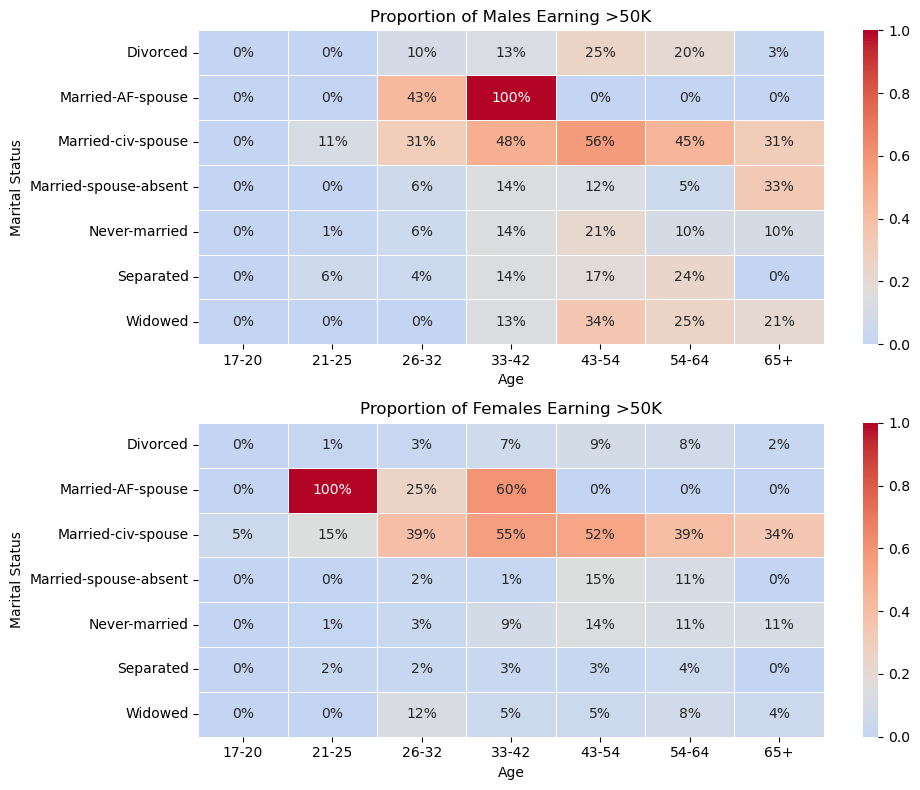
\includegraphics[width=1.05\linewidth]{mf_marital_agebins.png}  % Reduce width slightly
    \caption{Male and Female Salary by Marital Status vs Age}
    \label{fig:mf_marital_agebins}
\end{figure}


\textbf{Visual Analysis:} 
\medskip
    
\underline{\textbf{Males}}

The highest earning male group appears in the 43-54 age range.
Being married by age 25 seems to be a strong indicatory of future high salaries.
This suggests that marriage and middle age are strong correlates of higher income for men.
Being divorced or widowed seems to impair men's ability to earn a high salary down substantially.

\underline{\textbf{Females}}

For females, being married to a civilian spouse (Married-civ-spouse) is also a strong predictor of high income.
The highest income proportion is in the 26-50 range, peaking at around 54\%.
The divorced, widowed, and separated categories show especially weak salary trends.
Married-spouse-absent and never-married have somewhat of a bump compared to these groups (15\% versus 3-9\%).

However, compared to males, even married women earning a high salary is less common.


\underline{\textbf{Both}}

Males and Females who are married (Married-civ-spouse) show the highest proportion of high earners.


Males in the 33-42 age range who are Married-AF-spouse and Females who are 21-25 and Married-AF-spouse
show an extremely high proportion (~1.0) of earners above 50K. However, this may be due to low sample size rather than a strong trend. 

\textbf{User Story 2:} A group of UVW Foreign relations researchers would like us to compare income variations among individuals based on their native country and work class.

\textbf{Variable Analysis:} When analyzing our dataset, we found that the number of people surveyed with `native-country' as United-States vastly overwhelms the rest of the data. 
Therefore, we did a probability analysis to see those earning 50K or more as a percentage of each country's population. The number of countries is also very high and
the tail of the dataset becomes very narrow, meaning that we don't have a ton of samples to look at from less common countries. 
We took the U.S. and the top 5 most common countries in the dataset outside of the U.S. and combined them into one graph. 
Since this is proportional to earning salary, we removed the `without-pay' and `never-worked' columns to reduce visual clutter.
Then, our hue became `workclass' to meet the requirements of the user story.

\begin{figure}[h]
    \centering
    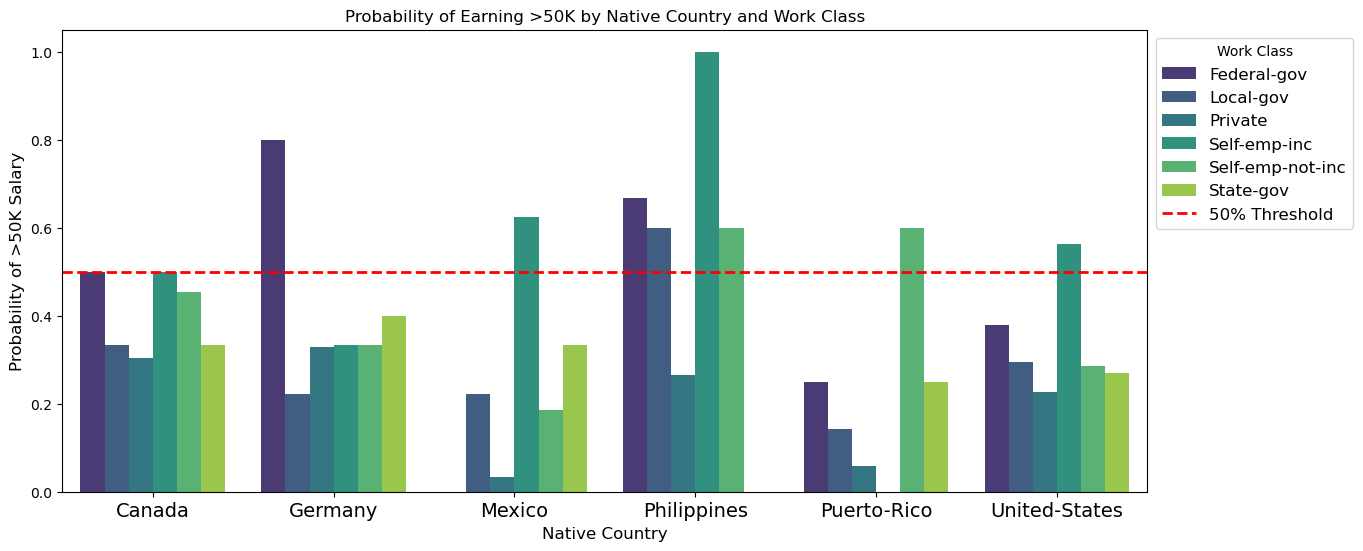
\includegraphics[width=1.05\linewidth]{country-workclass.png}  % Reduce width slightly
    \caption{Male and Female Salary by Marital Status vs Age}
    \label{fig:mf_marital_agebins}
\end{figure}

\textbf{Visual Analysis:} 

\medskip

The probability of earning more than $50K$ varies significantly across work classes and countries. The 50\% threshold line (red dashed line) serves as a key benchmark to determine which groups are more likely to be high earners.
Self-employed incorporated (self-emp-inc) consistently ranks high, often surpassing the 50\% threshold across multiple countries.
Government jobs (federal-gov, state-gov, and local-gov) display moderate earnings probabilities, often hovering around 40-60\%.
Private-sector employees (private) show variability, with some countries having significantly higher probabilities than others.
Self-employed but not incorporated (self-emp-not-inc) has a wider spread, showing both strong and weak earning probabilities depending on the country.

\medskip

\textbf{Country-Specific Insights}

\medskip

\underline{United States:}
\par A high proportion of self-emp-inc individuals surpass the 50\% threshold, making it one of the strongest predictors of high earnings.
Government jobs (particularly federal-gov) also perform well, but local and state government roles show a more balanced distribution below the 50\% mark.
Private-sector workers are more evenly split, with some hovering around 50\% and others falling below.

\underline{Canada, Germany:}
\par Canada and Germany have similar trends in which self-emp-inc and federal-gov workers are among the highest earners.
Local and state government jobs are more stable, but fewer exceed 50\%.
Private workers fall behind self-employed incorporated individuals, but they still maintain reasonable earning probabilities.

\underline{Mexico, Puerto Rico:}
\par Mexico exhibits the lowest earning probabilities overall, with many work classes failing to cross the 50\% threshold.
Puerto Rico has a notable self-emp-inc category that surpasses 50\%, while government positions and private jobs show a more even split.

\underline{Philippines:}
\par The strongest self-employment signals come from the Philippines, where self-employed incorporated (self-emp-inc) individuals have the highest probability of earning >50K across all countries in this dataset.
Federal and state government jobs perform well, reaching around 50\%.
Private-sector workers show more variance, with many remaining below the 50\% mark.

\medskip

\textbf{Key Observations}

Self-employed incorporated (self-emp-inc) is the strongest predictor of high earnings across almost all countries.
Federal government jobs are generally stable, often sitting around the 50\% threshold.
State and local government jobs have greater variation, often falling below 50\% in certain countries.
Private-sector employees display country-dependent variation, with some earning probabilities exceeding 50\% while others remain lower.
Mexico and Puerto Rico have the lowest high-earning probabilities overall, with Mexico showing the weakest upward trend.

\medskip

\textbf{User Story 3:} Workforce development strategist is asking us to to 
compare income variations among individuals based on their sex and hours worked

\textbf{Variable Analysis:} We created a box plot for this analysis to compare 
income variations among individuals based on their sex and hours worked per week.
This visualization was chosen because it effectively displays distribution,
median work hours, interquartile range (IQR), and outliers, allowing us
to simply observe differences between less than 50K and greater than 50K earners. The x-axis
represents hours worked per week, while the y-axis categorizes individuals by income group
in two region,with hue distinguishing between males and females.
The design process involved filtering relevant data and selecting a meaningful
color palette (blue for males and pink for females), and adjusting figure size
and median line thickness to enhance readability.

\begin{figure}[h]
    \centering
    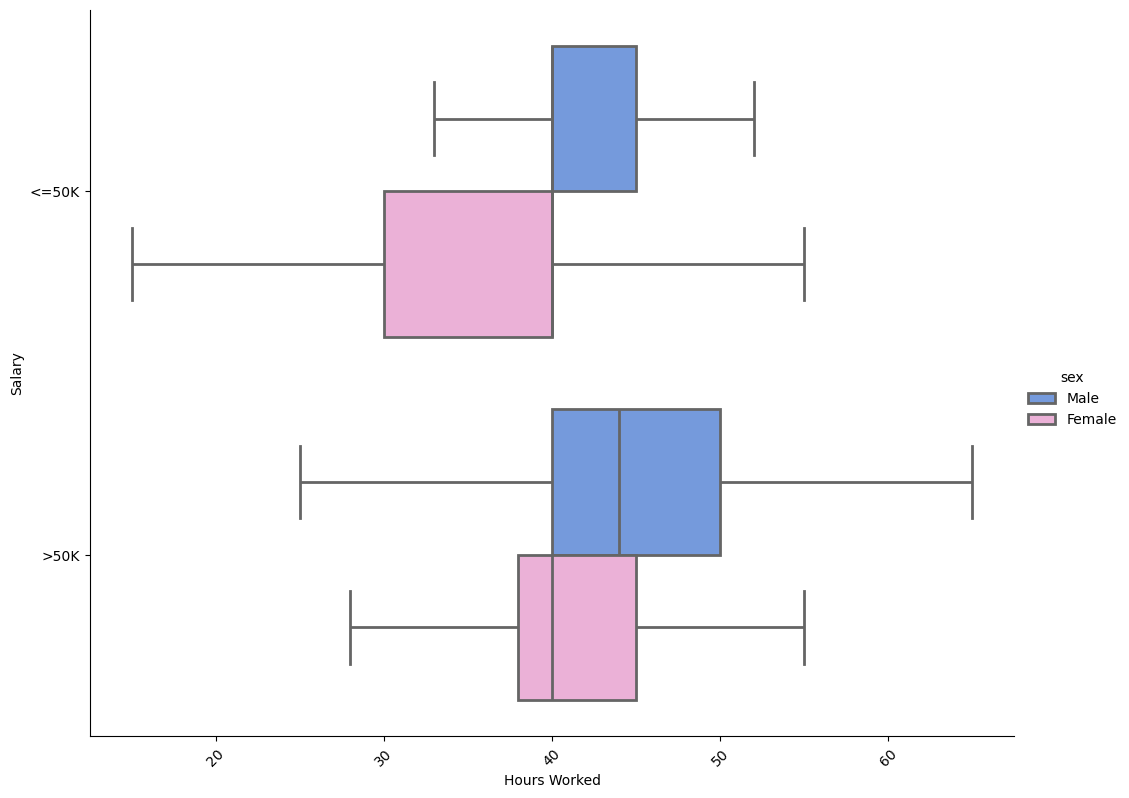
\includegraphics[width=0.9\linewidth]{gender_hours.png}  % Reduce width slightly
    \caption{Final histogram for Income vs Education}
    \label{fig:final_income_vs_education}
\end{figure}

\textbf{Visual Analysis:} 
The plot reveals that higher-income individuals generally work more hours, 
but males tend to have a wider spread in work hours compared to females, 
especially in the >50K group. Additionally, there are more outliers among high-earning men,
indicating cases of extreme work hours (60+ per week). 
In contrast, lower-income individuals exhibit a more compact work-hour distribution.

The result is a clear comparison of how work hours and income interact 
across genders, providing insights into employment trends for workforce development strategists.

\textbf{User Story 4:} Capital gains vs Occupation vs Salary
\textbf{Variable Analysis:} 
We created a histogram to analyze the distribution of capital-gain across
individuals earning <=50K and >50K. This visualization was chosen because
capital gains are highly skewed, with most individuals reporting zero or
small values, while a few report very high values. To improve interpretability,
we filtered the data to exclude individuals with zero capital-gain and
those with gains exceeding \$45,000, which may be extreme outliers.
The histogram uses hue to differentiate between salary groups, allowing us to compare distributions directly.
The spikes at specific capital-gain values (e.g., 10,000, 7,298, and 3,103) suggest that some
individuals report standard rounded amounts rather than varied capital gains,
possibly due to tax reporting practices or employer-based stock gains.
The plot also reveals that high capital gains are disproportionately associated
with the >50K income group, whereas <=50K earners rarely report significant
capital gains. The design process involved data filtering, selecting an
appropriate bin range, and adjusting the color palette (blue for >50K, orange for <=50K)
to enhance clarity. This visualization provides insights into how capital
gains serve as a strong predictor of high-income individuals and may
reflect investment-based earnings rather than traditional wages.

\begin{figure}[h]
    \centering
    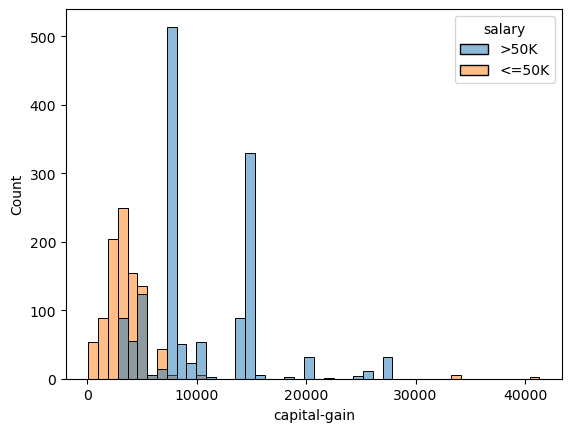
\includegraphics[width=0.9\linewidth]{capital-gain.png}  % Reduce width slightly
    \caption{Final histogram for Income vs Education}
    \label{fig:final_income_vs_education}
\end{figure}

\textbf{Visual Analysis:} 


\textbf{User Story 5:} A foreign relations researcher is interested in
understanding how capital gains vary based on relationship status
and whether this impacts income classification (<=50K vs. >50K).
By analyzing this interaction, we aim to identify potential patterns
in wealth accumulation and financial benefits associated with different
relationship categories.
\textbf{Variable Analysis:} 

For this analysis, we used a point plot to examine the relationship between
capital gain, relationship type, and salary category. The x-axis represents
different relationship categories, while the y-axis displays capital gain.
The hue differentiates between individuals earning <=50K and those earning
>50K, allowing for a direct comparison. Capital gain is an important
financial metric as it reflects non-salary earnings such as stock sales,
dividends, or real estate profits. This visualization helps us determine
whether certain relationship groups tend to accumulate more capital gains
and how that correlates with their overall income classification.

The design process for this visualization involved choosing a point plot
because it effectively displays central tendencies and variability for
a continuous variable (capital gain) across multiple categorical groups
(relationship status). The color scheme (blue for <=50K, orange for >50K)
enhances clarity, and the error bars help us assess the spread and
reliability of the data in each category.

\begin{figure}[h]
    \centering
    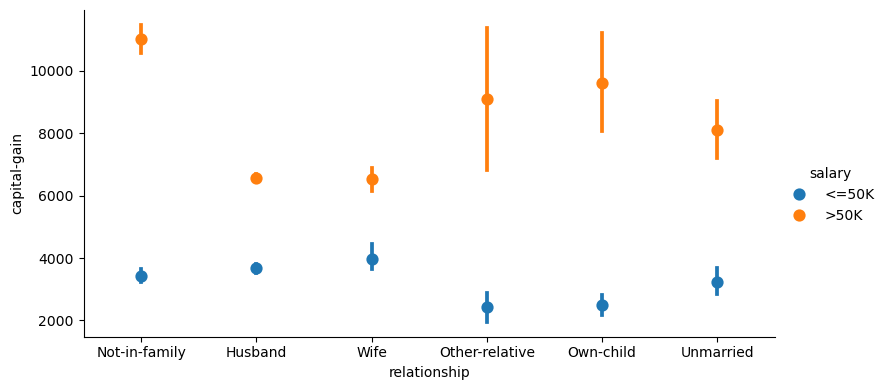
\includegraphics[width=0.9\linewidth]{capital-gain-relationship.png}  % Reduce width slightly
    \caption{Final histogram for Income vs Education}
    \label{fig:final_income_vs_education}
\end{figure}


\textbf{Visual Analysis:} 

Individuals classified as “Husband” have the highest median capital gains among >50K earners, significantly outpacing all other groups. This suggests that married men (likely filing jointly) may have more access to investment income.
“Wife” also shows notable capital gains, but at lower levels compared to “Husband,” possibly due to gender-based earning disparities.
“Own-child,” “Unmarried,” and “Other-relative” categories show high variability in capital gain distribution but tend to have a lower median capital gain overall. This may indicate that these groups have fewer investment-based earnings, relying more on salary income.
For individuals earning <=50K, capital gains remain near zero across all relationship groups, confirming that significant capital gains are predominantly associated with high-income individuals.
The large error bars for some categories (e.g., “Own-child”) suggest high variability and potentially small sample sizes in those groups.

Overall, this visualization demonstrates that capital gains are strongly associated with high-income earners, particularly among married individuals (husbands and wives), while lower-income groups tend to report negligible capital gains.

\section{Appendix}
\end{document}
